%! Author = itgramic
%! Date = 29.12.23

% Preamble
\subsubsection{Anforderungen}
\begin{flushleft}
    Das KSGR hat eine Cloud First Strategie.\\
    Das heisst, alle neuen Applikationen und entsprechend deren Datenbanken müssen Cloud Ready bzw.
    Cloud Native sein.
    Um die Voraussetzung dafür zu schaffen, muss auch der PostgreSQL Cluster Cloud Ready sein.
\end{flushleft}
\begin{flushleft}
    Daher müssen zwei von drei genauer evaluierten Lösungen Cloud Native Lösungen sein.
    Wenn der Zeitaufwand reicht, können auch eine Cloud Native und Monolithisches System aufgebaut werden.
\end{flushleft}
\begin{flushleft}
    \begin{landscape}
    {\small
\begin{longtable}[H]{rlllll}
 \hdashline
\toprule
Nr. & Anforderung & Bezeichnung & Beschreibung & System & Muss / Kann \\ \hdashline
\midrule
\endfirsthead
\caption[]{Anforderungskatalog} \\ \hdashline
\toprule
Nr. & Anforderung & Bezeichnung & Beschreibung & System & Muss / Kann \\ \hdashline
\midrule
\endhead
\midrule
\multicolumn{6}{r}{Continued on next page} \\ \hdashline
\midrule
\endfoot
\bottomrule
\endlastfoot
1 & Systemvielfallt &  & \begin{tabular}[c]{@{}l@{}}Es muss mindestens eine Monolitisches und mindestens 2 zwei Distributed SQL Cluster ermittelt werden.\end{tabular} & Beides & MUSS \\ \hdashline
2 & Synergien &  & \begin{tabular}[c]{@{}l@{}}Skripte und APIs des Monolithisches Systems müssen auch in einem Distributed SQL System verwendet werden können.\end{tabular} & Beides & MUSS \\ \hdashline
3 & Failover & Automatismus & \begin{tabular}[c]{@{}l@{}}Das Clustersystem muss bei einem Nodeausfall automatisch auf einen anderen Node umstellt werden.\end{tabular} & Beides & MUSS \\ \hdashline
4 & Failover & Connection - Stabilität & \begin{tabular}[c]{@{}l@{}}Beim Failover dürfen bestehende Connections nicht getrennt oder sofort wiederhergestellt werden.\end{tabular} & Beides & MUSS \\ \hdashline
5 & Failover & Geschwindigkeit & \begin{tabular}[c]{@{}l@{}}Das Umstellen auf den nächsten Node muss so schnell ausgeführt werden,\\damit ein Disconnect mittels Client-Konfiguration (Timeout) verhindert wird.\end{tabular} & Beides & MUSS \\ \hdashline
6 & Switchover & Skript / API & \begin{tabular}[c]{@{}l@{}}Das System muss ein Skript oder eine API liefern,\\welche einen geordeten Switchover auf einen anderen Node erlaubt.\end{tabular} & Beides & MUSS \\ \hdashline
7 & Switchover & Connection - Stabilität & \begin{tabular}[c]{@{}l@{}}Beim Switchover dürfen bestehende Connections nicht getrennt werden oder sofort wiederhergestellt werden.\end{tabular} & Beides & MUSS \\ \hdashline
8 & Switchover & Geschwindigkeit & \begin{tabular}[c]{@{}l@{}}Das Umstellen auf den nächsten Node muss so schnell ausgeführt werden,\\das ein Disconnect mittels Client-Konfiguration (Timeout) verhindert wird.\end{tabular} & Beides & MUSS \\ \hdashline
9 & Restore & Skript / API & \begin{tabular}[c]{@{}l@{}}Das Clustersystem muss ein Skript oder eine API liefern,\\welche das einfache und ggf. automatisierte Restoren eines oder mehreren Nodes ermöglichen.\end{tabular} & Beides & MUSS \\ \hdashline
10 & Restore & Datensicherheit & \begin{tabular}[c]{@{}l@{}}Beim Wiederherstellen des Ursprungszustands darf es zu keinem Datenverlust kommen.\end{tabular} & Beides & MUSS \\ \hdashline
11 & Restore & Connection - Stabilität & \begin{tabular}[c]{@{}l@{}}Bei der Wiederherstellung einzelner Nodes darf es zu keinen Unterbrechungen auf den Applikationen kommen.\end{tabular} & Beides & MUSS \\ \hdashline
12 & Restore & Geschwindigkeit & \begin{tabular}[c]{@{}l@{}}Das Wiederherstellen des Ursprungszustands muss\\innert weniger Stunden für alle Datenbanken aus dem\\Backup wiederhergestellt und im Clustersystem synchronisiert werden.\end{tabular} & Beides & MUSS \\ \hdashline
13 & Replikation & Synchrone Replikation & \begin{tabular}[c]{@{}l@{}}Es muss eine synchrone Replikation sichergestellt werden.\end{tabular} & Monolitisch & MUSS \\ \hdashline
14 & Replikation & Failover / Switchover Garantie & \begin{tabular}[c]{@{}l@{}}Die Replikation muss sicherstellen, das es bei einem Failover/Switchover zu keinem Fehler kommt\end{tabular} & Monolitisch & MUSS \\ \hdashline
15 & Replikation & Throughput & \begin{tabular}[c]{@{}l@{}}Beschreibt, wie viele Transaktionen pro Zeiteinheit vom Primary an die Replikas gesendet und Commited werden.\\Dieser Wert ist bei synchroner Replikation entscheidend, da Commits auf allen Replicas abgesetzt sein müssen.\end{tabular} & Beides & MUSS \\ \hdashline
16 & Sharding & Datenschutz- und integrität & \begin{tabular}[c]{@{}l@{}}Die Datenkonsistenz und Datenintegrität auf den Shards muss sichergestellt werden.\end{tabular} & Distributed SQL & MUSS \\ \hdashline
17 & Sharding & Schutz vor Datenverlust & \begin{tabular}[c]{@{}l@{}}Die Synchronisation der Shards muss sicherstellen, dass es zu keinem Datenverlust kommt.\end{tabular} & Distributed SQL & MUSS \\ \hdashline
18 & Quorum & Quorum-System vorhanden & \begin{tabular}[c]{@{}l@{}}Das Clustersystem muss über ein Quorum-System besitzen.\end{tabular} & Beides & MUSS \\ \hdashline
19 & Quorum & Robhustheit & \begin{tabular}[c]{@{}l@{}}Das Quorum des Clustersystems muss robust genug sein, um eine Split-Brain-Situation zu verhindern.\end{tabular} & Beides & MUSS \\ \hdashline
20 & Connection &  & \begin{tabular}[c]{@{}l@{}}Das Clustersystem muss sicherstellen,\\dass eine Applikation ohne Entwicklungsaufwand mittels dem PostgreSQL Wired Connector zugreifen kann.\end{tabular} & Beides & MUSS \\ \hdashline
21 & Management-API & Management-API vorhanden & \begin{tabular}[c]{@{}l@{}}Das Clustersystem muss Skripte oder eine API liefern,\\mit denen sich das System konfiguriert, verwaltet oder überwacht werden kann.\\Zudem müssen mit geringen Arbeitsaufwand Nodes hinzugefügt oder entfernt werden können.\end{tabular} & Beides & MUSS \\ \hdashline
22 & Management-API & Authentifizierung \& Autorisierung & \begin{tabular}[c]{@{}l@{}}Es müssen gängige Standards für Authentifizierung und Autorisierung mitgebracht werden.\end{tabular} & Beides & MUSS \\ \hdashline
23 & Management-API & Aufwand & \begin{tabular}[c]{@{}l@{}}Der Aufwand,\\der benötigt wird, um die DB zu verwalten,\\Nodes hinzuzufügen oder zu entfernen usw., muss gegeneinander verglichen werden.\end{tabular} & Beides & MUSS \\ \hdashline
24 & Backup & Backup mit PostgreSQL Standards & \begin{tabular}[c]{@{}l@{}}Backups müssen mittels PostgreSQL Standards angezogen werden können.\end{tabular} & Beides & MUSS \\ \hdashline
25 & Backup & Restore mit PostgreSQL Standanrds & \begin{tabular}[c]{@{}l@{}}Backups müssen mittels PostgreSQL Standards restored werden können\end{tabular} & Beides & MUSS \\ \hdashline
26 & Housekeeping - Log Rotation &  & \begin{tabular}[c]{@{}l@{}}Das Clustersystem muss die Möglichkeit zur Log Rotation bieten.\end{tabular} & Beides & MUSS \\ \hdashline
27 & Self Heahling &  & \begin{tabular}[c]{@{}l@{}}Das Clustersystem muss im Fehlerfall Nodes selber wiederherstellen können.\end{tabular} & Beides & KANN \\ \hdashline
28 & Monitoring - Node Failure &  & \begin{tabular}[c]{@{}l@{}}Läuft ein Node auf einen Fehler,\\muss das Clustersystem dies erkennen und melden resp.\\eine Schnittstelle liefern, die abgefragt werden kann.\end{tabular} & Beides & MUSS \\ \hdashline
29 & Maintenance Quality &  & \begin{tabular}[c]{@{}l@{}}Da die meisten PostgreSQL HA Lösungen Open-Source sind, muss sichergestellt werden,\\dass die gewählte Lösung auch aktiv gepflegt wird.\\Als Basis dient GitHub Insights.\end{tabular} & Beides & MUSS \\ \hdashline
30 & Performance & tps - Read-Only & \begin{tabular}[c]{@{}l@{}}Die Transaktionsrate (transactions per second / tps) für DQL Transaktionen.\end{tabular} & Beides & MUSS \\ \hdashline
31 & Performance & tps - Read-Writes & \begin{tabular}[c]{@{}l@{}}Die Transaktionsrate (transactions per second / tps) für DML Transaktionen.\end{tabular} & Beides & MUSS \\ \hdashline
32 & Performance & Ø Latenz - Read-Only & \begin{tabular}[c]{@{}l@{}}Die Latenzzeit bei DQL Transaktionen.\end{tabular} & Beides & MUSS \\ \hdashline
33 & Performance & Ø Latenz - Read-Write & \begin{tabular}[c]{@{}l@{}}Die Latenzzeit bei DML Transaktionen.\end{tabular} & Beides & MUSS \\ \hdashline
\caption{Anforderungskatalog} \label{anforderungskatalog}
\end{longtable}

}
    \end{landscape}
\end{flushleft}
%\begin{flushleft}
%    \begin{description}
%        \item \textbf{Kostenrechnung}\hfill \\Für die Kostenberechnung des Zeitaufwands wird im KSGR intern mit \(120CHF/h\) gerechnet.\\Jeder Arbeitstag hat dabei \(8.4h\) und pro Jahr wird mit \(220 Tagen\) gerechnet.
%        \item \textbf{Messung des Zeitaufwands}\hfill \\Der Zeitaufwand in der Evaluationsphase kann nur mit manueller Ausführung gemessen werden, da die Automatisierung nicht in der Evaluationsphase umgesetzt werden kann.\\In die Evaluation einfliessen wird aber die Schätzung, wie viel Aufwand betrieben werden muss um die wichtigsten Tasks automatisieren zu können.
%        \item
%    \end{description}
%
%    Folgende Messgrössen werden gestellt:
%    \begin{description}
%        \item \textbf{Quorum}\hfill \\
%        \item \textbf{Zeitaufwand Quorum erweitern}\hfill \\Bemessen wird, wie lange man braucht um einen neuen Node dem Quorum hinzuzufügen.
%        \item \textbf{Zeitaufwand Failover und Recovery}\hfill \\Bemessen wird, wie lange ein Failover und ein anschliessender Recover auf den normalen Zustand dauert.
%        \item \textbf{Failover Funktionsfähigkeit}\hfill \\Misst, ob der Failover bei korrekter Konfiguration funktionsfähig ist wie er vom entsprechenden System spezifiziert wurde.
%        \item \textbf{Failover Reaktionszeit}\hfill \\Gemessen und bemessen wird, wie lange es im Failoverszenario dauert, bis auf einen Standby-Node umgeschaltet wird und wie lange es dauert bis offene Connections wieder voll funktionsfähig sind.
%        \item \textbf{Recoverydauer}\hfill \\Bemisst, wie lange es nach einem Failover-Szenario dauert, bis der Normalzustand Widerhergestellt werden kann.
%    \end{description}
%
%
%\end{flushleft}
\subsubsection{Stakeholder}
\begin{table}[H]

\resizebox{\columnwidth}{!}{%

\begin{tabular}{lllll}
\toprule
Rolle & Funktion & Departement & Bereich & Abteilung \\
\midrule
Zabbix Stakeholder & Abteilungsleiter  & D10 ICT & Infrastrukturmanagement & ICT Netzwerk, Security und Comm. \\
Staekholder Data Center Infrastruktur & Abteilungsleiter  & D10 ICT & Infrastrukturmanagement & ICT Data Center \\
k8s Stakeholder & ICT System Ingenieur & D10 ICT & Infrastrukturmanagement & ICT Data Center \\
\bottomrule
\end{tabular}
}
\caption{Stakeholder} \label{stakeholder}
\end{table}

\begin{flushleft}
\end{flushleft}
\subsubsection{Gewichtung}
\begin{flushleft}
    Die Gewichtung wurde mittels einer Präferenzmatrix ermittelt.\\
    Dabei wurden folgende Anforderungen aus übersichtsgründe in Sub-Matrizen aufgeteilt:
    \begin{description}
        \item Failover
        \item Switchover
        \item Restore
        \item Replikation
        \item Sharding
        \item Quorum
        \item Management-IP
        \item Backup
        \item Performance
    \end{description}

    Die Grundlegende Gewichtung wurde folgendermassen vorgenommen:
    \begin{figure}[H]
        \centering
        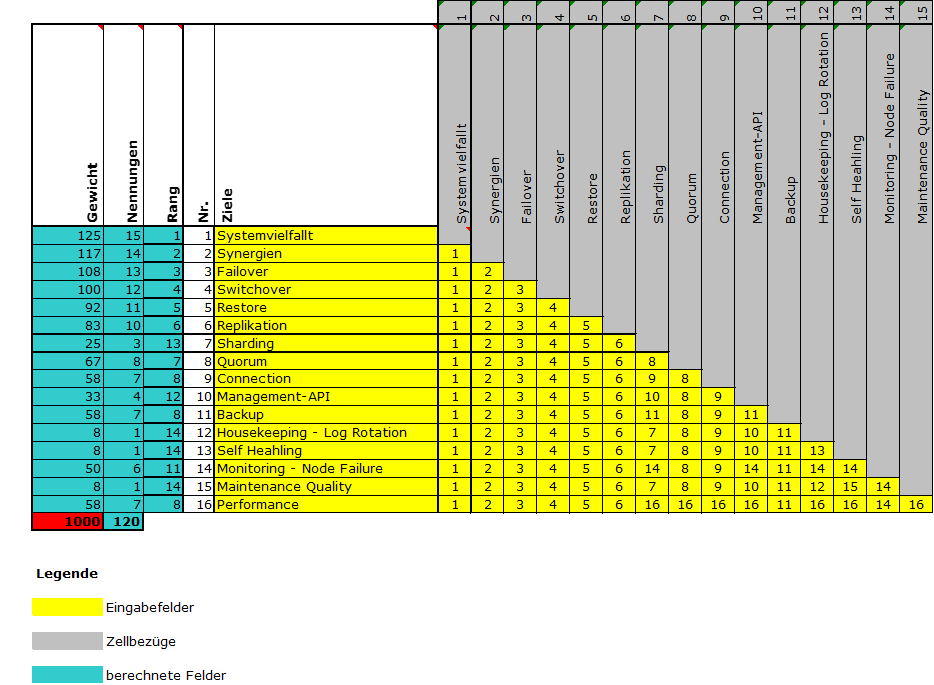
\includegraphics[width=1\linewidth]{source/implementation/evaluation/requirements/preference_matrix}
        \caption{Präferenzmatrix}
        \label{fig:preference_matrix}
    \end{figure}
\end{flushleft}
\begin{flushleft}
    Die Gewichtung der Failover-Anforderungen setzt sich wie folgt zusammen:
    \begin{figure}[H]
        \centering
        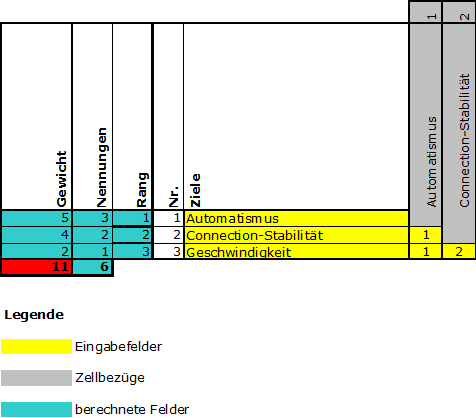
\includegraphics[width=0.75\linewidth]{source/implementation/evaluation/requirements/preference_matrix_failover}
        \caption{Präferenzmatrix - Failover}
        \label{fig:preference_matrix_failover}
    \end{figure}
\end{flushleft}
\begin{flushleft}
    Beim Switchover wurde die Gewichtung wie folgt aufgeteilt:
    \begin{figure}[H]
        \centering
        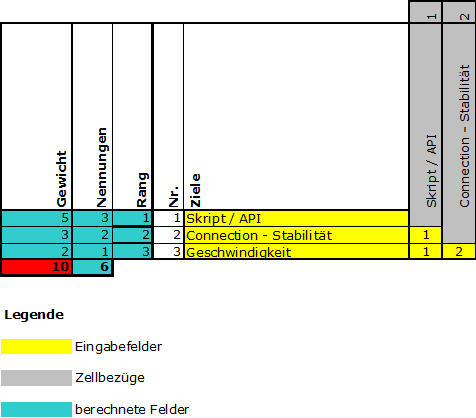
\includegraphics[width=0.75\linewidth]{source/implementation/evaluation/requirements/preference_matrix_switchover}
        \caption{Präferenzmatrix - Switchover}
        \label{fig:preference_matrix_switchover}
    \end{figure}
\end{flushleft}
\begin{flushleft}
    Die Gewichtung und Aufteilung der Restore-Anforderungen sieht wie folgt aus:
    \begin{figure}[H]
        \centering
        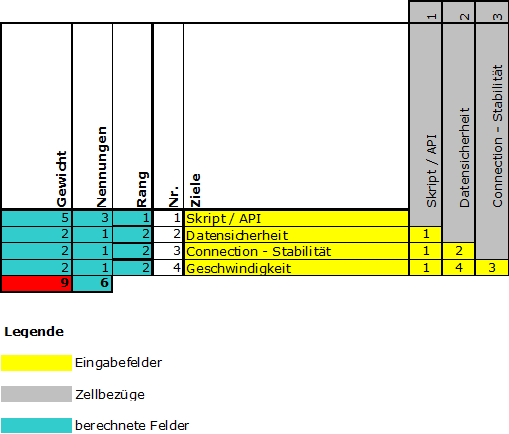
\includegraphics[width=0.75\linewidth]{source/implementation/evaluation/requirements/preference_matrix_restore}
        \caption{Präferenzmatrix - Restore}
        \label{fig:preference_matrix_restore}
    \end{figure}
\end{flushleft}
\begin{flushleft}
    Die Replikationsanforderungen resp.
    deren Gewichtung ist wie folgt aufgebaut:
    \begin{figure}[H]
        \centering
        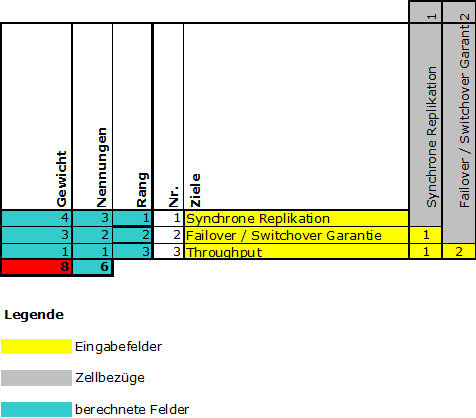
\includegraphics[width=0.75\linewidth]{source/implementation/evaluation/requirements/preference_matrix_replication}
        \caption{Präferenzmatrix - Replikation}
        \label{fig:preference_matrix_replication}
    \end{figure}
\end{flushleft}
\begin{flushleft}
    Das Sharding setzt sich aus folgenden Teilen zusammen:
    \begin{figure}[H]
        \centering
        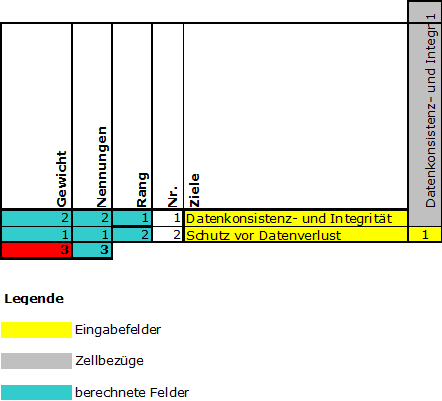
\includegraphics[width=0.75\linewidth]{source/implementation/evaluation/requirements/preference_matrix_sharding}
        \caption{Präferenzmatrix - Sharding}
        \label{fig:preference_matrix_sharding}
    \end{figure}
\end{flushleft}
\begin{flushleft}
    Die Quorum-Anforderung ist folgendermassen zusammengesetzt:
    \begin{figure}[H]
        \centering
        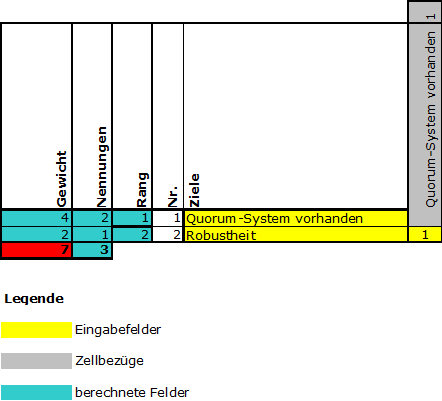
\includegraphics[width=0.75\linewidth]{source/implementation/evaluation/requirements/preference_matrix_quorum}
        \caption{Präferenzmatrix - Quorum}
        \label{fig:preference_matrix_quorum}
    \end{figure}
\end{flushleft}
\begin{flushleft}
    Bei der Management-API gibt es mehrere Sub-Anforderungen:
    \begin{figure}[H]
        \centering
        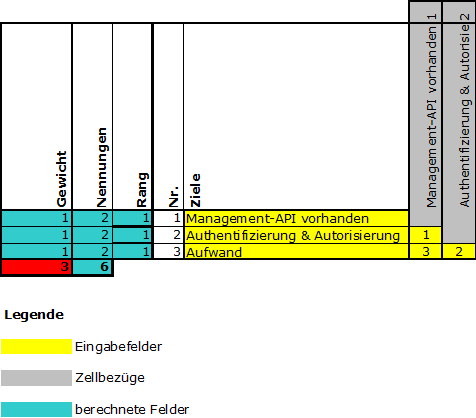
\includegraphics[width=0.75\linewidth]{source/implementation/evaluation/requirements/preference_matrix_management_api}
        \caption{Präferenzmatrix - Management-API}
        \label{fig:preference_matrix_management_api}
    \end{figure}
\end{flushleft}
\begin{flushleft}
    Anforderungen zum Backup wurden nachfolgend aufgeteilt und gewichtet:
    \begin{figure}[H]
        \centering
        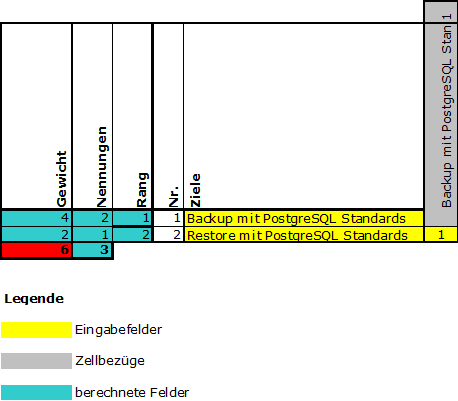
\includegraphics[width=0.75\linewidth]{source/implementation/evaluation/requirements/preference_matrix_backup}
        \caption{Präferenzmatrix - Backup}
        \label{fig:preference_matrix_backup}
    \end{figure}
\end{flushleft}
\begin{flushleft}
    Performance-Benchmarking lässt sich in nachfolgende Teile unterteilen:
    \begin{figure}[H]
        \centering
        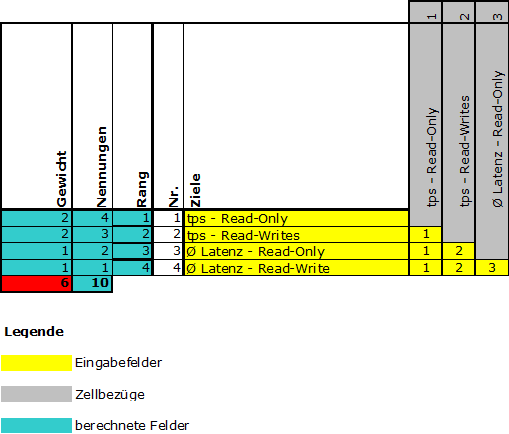
\includegraphics[width=1\linewidth]{source/implementation/evaluation/requirements/preference_matrix_performance}
        \caption{Präferenzmatrix - Performance}
        \label{fig:preference_matrix_performance}
    \end{figure}
\end{flushleft}